%%% -*-LaTeX-*-

\chapter{Introduction}

Understanding the behaviour of flows\footnote{All packets with the same source/destination IP address, source/destination ports, protocol interface and class of service are grouped into a flow.} at port level is well studied whereas understanding the behaviour of hosts and groups of hosts is less well studied. The latter in conjunction with the former is helpful to network admins in making informed decisions in day to day activities. Network administrators perform various network mangement activities and equipping them with right information will lead to better performance. 
Our system analyzes daily network data and extracts host\footnote{A host in our system is defined as any unique IP address.} behaviors out of it.  Behavior of a host is an aggregate of the amount of traffic that it sends both in terms of packets and bytes, the set of destinations it tries to connect to , the set of protocols it uses over some time period. For the purposes of our study the time period that we choose is a day. There is nothing inherent about choosing day as a time frame but we expect that the way networks are used varies from the days to nights and a day would be long enough to capture all these variations. These behaviors help us in learning more about what is going in the network. Presently, admins use the following techniques to manage networks. 
\begin{itemize}
	\item They perform aggregation based on ports, protocols, applications. This helps in identifying applications consuming the most bandwidth, ports that are being used heavily, consolidate flow data from multiple devices, monitor wireless network bandwidth.	
	\item They perform deep packet inspection to know what is in the payload of a packet. This is generally performed to extract the urls or sites that users are  visiting. This is a fine grained version of the above technique.	
	\item Rule based systems are generally incorporated by admins to secure the network from malicious users. In a rule based system a trigger is executed when specific actions occur. An example would be blocking the IP address of the user if he has more than 6 unsuccessful login attempts. Here the action is six unsuccessful attempts and the trigger is blocking the IP address. 
\end{itemize}

\begin{figure}[b]
	\centerline{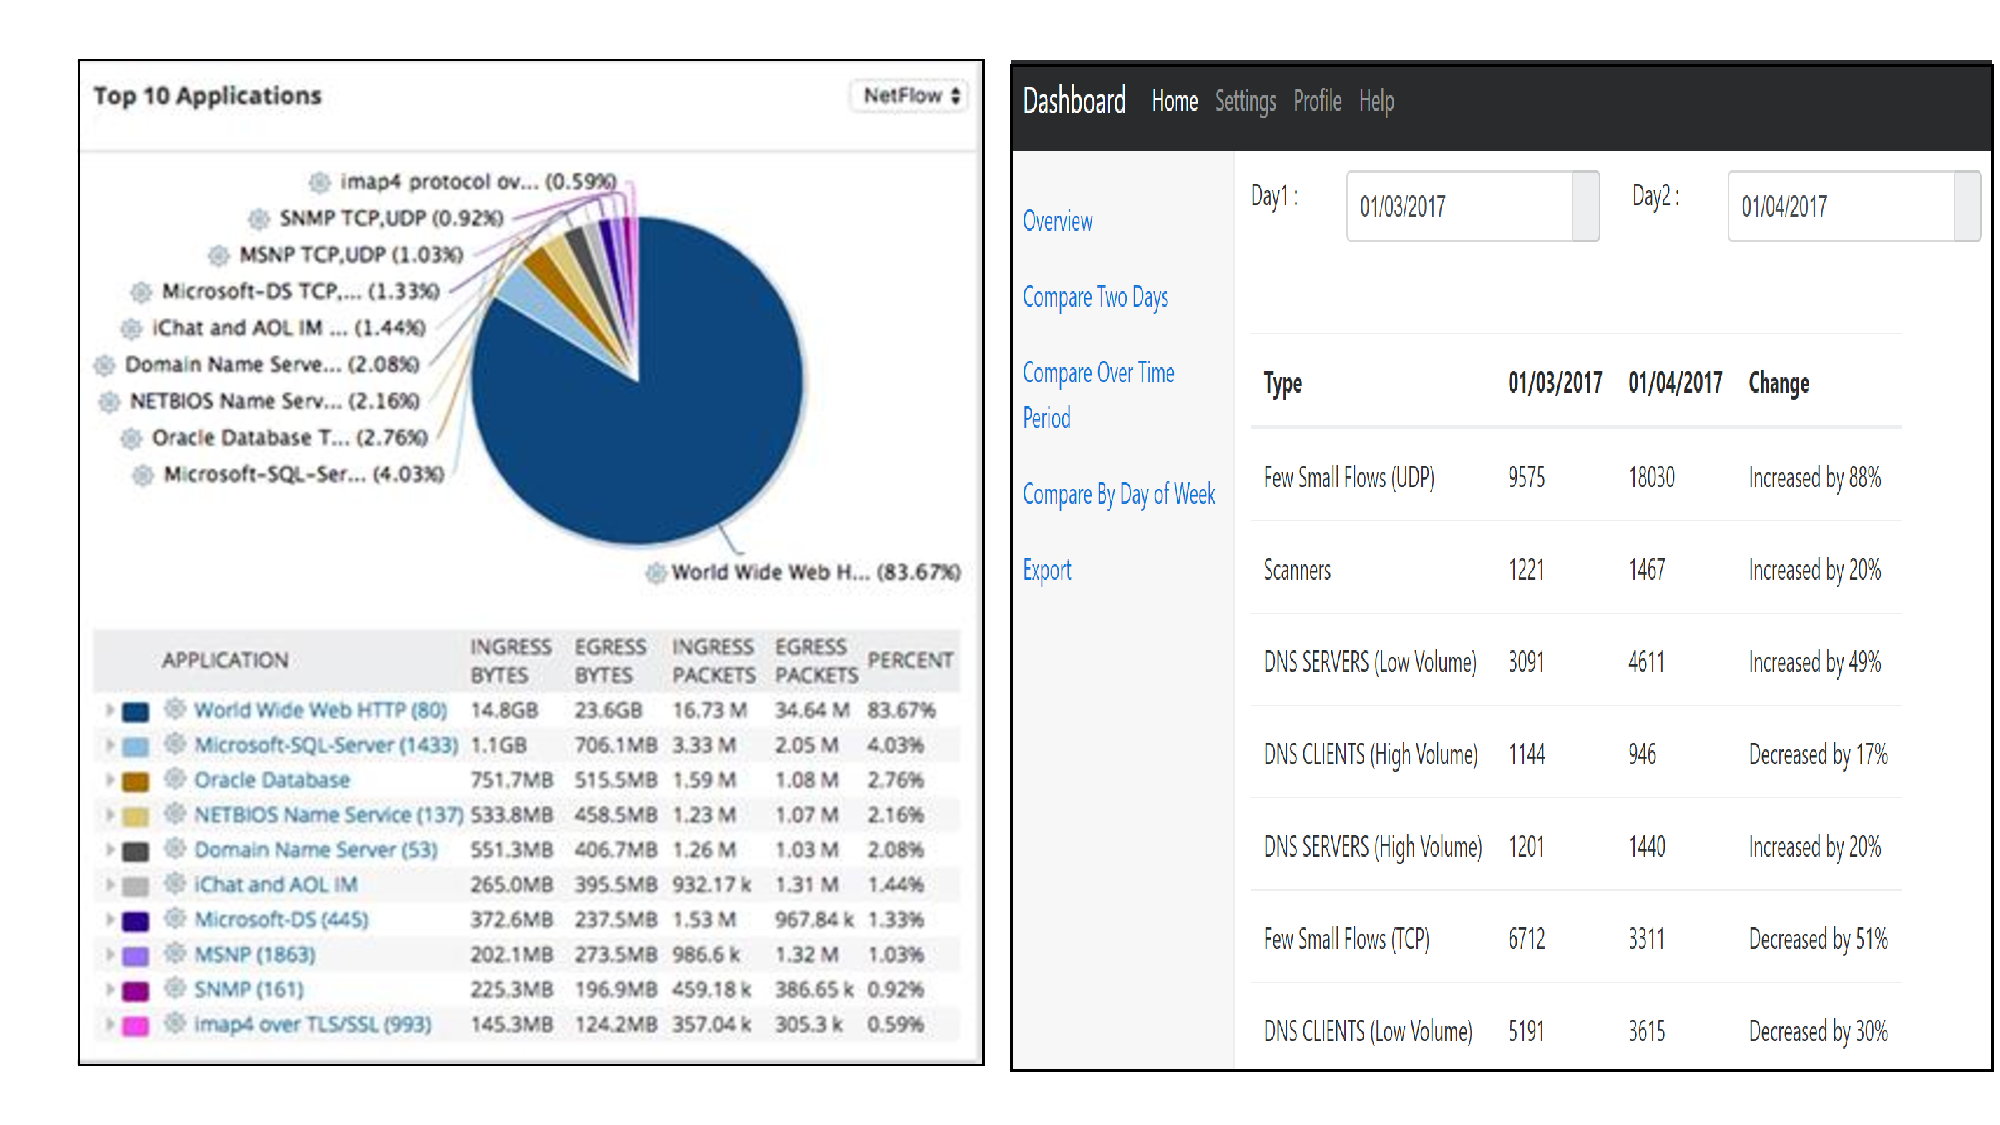
\includegraphics[scale = 0.5]{intro.pdf}}
	\caption{SolarWinds in comparison with our system}%
	\figlabel{intro}
\end{figure}

Now, let us look at how does the present techniques differ from our proposed work. In the \figref{intro} the left image represents a screenshot taken from Solarwinds\footnote{Solarwinds is an application that performs network monitoring using aggregation techniques when NetFlow data is passed as input.} application when our data is passed through it. Here we can clearly see that the SolarWinds tool listed top 10 applications being used. If we look at the blue colored section of the pie chart it says that 83.67 percent of the traffic is World Wide Web traffic on port 80. 

Moving on to the right side of the figure, it is a screenshot from the system we developed. Consider the hosts which are behaving as scanners on a Jan 3rd they were 1221 of them and on Jan 4th they are 1461 with an increase of 29 percent. One can clearly observe the difference between the two screenshots. While one views at the top applications and which ports make up the majority of traffic. The other views at the types of hosts and how they are changing over time. These are two different views of the same network data.

The obvious question that arises is why do we need an other view of network data and the answer is because the existing views are no more sufficient to perform different network management activites and our proposed approach helps in identifying behaviors that are not detected by traditional techniques. From the \figref{intro} in the aggregation based techniques on the left side we are able to know that 86 percent of the traffic is web based. But what do we know about the hosts that are originators of these traffic. There could be hosts which are doing both DNS and WWW traffic. There could be hosts that are performing minimal amount of web traffic to evade from an anomaly event that they are performing. This information is not obtained from the SolarWinds or any other tool that uses these aggregation techniques. This is where we want our system to complement these existing techniques by providing hosts behaviors. Also, a major issue in network traffic analysis is classifying and characterizing traffic. Performing an accurate classification is indeed essential in various respects, such as traffic control, application identification, defense against attacks, and anomaly detection.
However, they are often observed to fail, either because of packet encryption, arbitrary or dynamic port use, or because different protocols or utilizations employ the same single port.
We also claim that hosts behaving similarly require similar amount of network resources and host behavior extraction will be an efficient way for network admins to plan their network capacity compared to the present bandwidth monitoring techniques. Some behaviors that could be of interest to the network admins are:


\begin{itemize}
	\item If hosts are behaving as clients or servers. This gives admin a clear picture of how the network is being used and who are the major contributors to the traffic.
	\item If there are a group of hosts that exchange large number of packets containing small bytes then it is normal interactive traffic in the network.	
	\item If a group of hosts are sending data to a single host. This could be an example of off-site back ups and network admin can use this information to plan the bandwidth accordingly.
	\item If a group of hosts are trying to scan on multiple ports then it is highly likely that these could be users trying to infiltrate into the network and admins could take actions appropriately.
	
\end{itemize}


To extract these behaviors we have used data mining techniques. The reason for approaching these techniques is firstly the amount of data that we want to look into is huge. Secondly, we want to find behaviors/patterns a human may have not known to look in first place and data mining is a field of study that performs exactly the same task. It extracts patterns from a given data set and present it to the user in an understandable format. Specifically, we used an unsupervised approach called clustering to extract these behaviors. We also applied other data mining methods to measure the quality of our clustering and find the divergence of host behaviors over a given time.  


\section{Contributions} \label{contributions}
\textbf{"By combining clustering and other data mining techniques we can produce a view of host behaviors that helps network administrators to understand behavior of the networks. This system complements existing network analysis tools to ease network management."}

The following are the main contributions from this work which supports and provides evidence for the thesis statement.

1) We have built a system that uses data mining techniques to extract host behaviors from the given Netflow data.

2) We have built a tool to analyze the host behaviors in different dimensions and render it visually to help administrator take decisions.

3) We performed an extensive evaluation of our approach using
emulated enterprise network data. This evaluation
demonstrates the ability of our system to detect host behaviors under challenging conditions, and to scale to enterprise-sized networks.


The rest of this paper is structured as follows. Section 2 gives a background of data mining. Section 3 discusses related work and plugs our work into context. Section 4 presents the design of our system. Section 5 provides the implementation details, while  Section 6 evaluates our system  and demonstrates our claims. Finally, we outline items for future work in Section 7.
